% Funcion para poner imagenes que tienen nombre con underscore:
\newcommand{\imagenB}[2]{%
\includegraphics[width=#1\textwidth]{#2}
\endgroup}

\def\imagen{\begingroup
\catcode`\_=12
\imagenB}
% -----------------------------------------

En esta sección, se detallan los diferentes experimentos que realizamos para medir la eficiencia y resultados de los algoritmos implementados.

\subsection{Page Rank}

\subsubsection{Instancias de prueba}

Para generar grafos sobre los cuales experimentar tuvimos que obtener varias muestras.
Por un lado, se utilizaron recursos de SNAP (http://snap.stanford.edu/) para las instancias mas grandes de grafos que utilizamos para medir tiempo y la convergencia del algoritmo Page Rank.
Además, generamos instancias originales mediante las herramientas provistas por la cátedra otras extra generadas por nosotros.

\subsubsection{Convergencia del algoritmo}

Realizamos una serie de experimentos con el propósito de analizar la convergencia de la solución provista por el algoritmo a través de las iteraciones que el mismo realiza en su ciclo principal.\\
Para hacer esto, modificamos el algoritmo (no su procedimiento) con el fin de ir guardando las soluciones temporales en cada paso.\\
Con estos datos, medimos la Norma Manhattan (L1) entre las soluciones de cada par de iteraciones sucesivas, definida como:

\begin{center}
$L_1(x,y) = \sum\limits_{i=1}^n | x[i] - y[i] | $
\end{center}

Siendo $n$ la cantidad de nodos del grafo siendo estudiado, $x \in \mathbb{R}^{n}$ la solución del algoritmo en una iteración $j$ e $y \in \mathbb{R}^{n}$ la de la iteración $j+1$.\\
Esta es una forma intuitiva y logica de estudiar la convergencia, ya que al tomar la suma de los valores absolutos entre los componentes de cada vector, lo que realmente estamos haciendo es calcular cuanto varia la solución que estamos calculando a través de las iteraciones. Además, podemos asegurar que por el procedimiento de nuestro algoritmo esta diferencia va a ir disminuyendo, y cuando sea lo suficientemente chica el algoritmo va a terminar.

Estudiamos la convergencia a través de dos instancias de tamaño mediano-grande obtenidos de SNAP, mas precisamente:
\begin{itemize}
    \item Instancia 1: 6301 nodos y 20777 ejes.
    \item Instancia 2: 10876 nodos y 39994 ejes.
\end{itemize}
Por lo que podemos decir que son considerables y relativamente esparsas (por ejemplo, el primero podria tener cerca de 40 millones de ejes si fuera completo, teniendo en cuenta que es un grafo dirigido).\\
A su vez, fuimos variando el componente $c$ del algoritmo Page Rank entre 0.3, 0.6 y 0.9, el cual controla la importancia del viajero aleatorio, es decir, a menor $c$ aumenta la probabilidad de que el usuario vaya a una página aleatoria desde la actual.\\
Veamos los resultados:

\begin{center}
    \begin{tikzpicture}
    \begin{axis}[
        title={Instancia 1},
        xlabel={Iteraci\'on $i$},
        ylabel={$L_1(x_i,x_{i+1})$},
        scaled x ticks=false,
        scaled y ticks=false,
        enlargelimits=0.05,
        width=0.5\textwidth,
        height=0.5\textwidth,
        legend pos=north west
    ]
    \addplot[color=black] table[x=instancia,y=l1]{datos/pr-1-1-1.out};
    \addplot[color=red] table[x=instancia,y=l1]{datos/pr-1-1-2.out};
    \addplot[color=green] table[x=instancia,y=l1]{datos/pr-1-1-3.out};
    \legend{c = 0.3, c = 0.6, c = 0.9}
    \end{axis}
    \end{tikzpicture}
    \begin{tikzpicture}
    \begin{axis}[
        title={Instancia 2},
        xlabel={Iteraci\'on $i$},
        ylabel={$L1(x_i,x_i+1)$},
        scaled x ticks=false,
        scaled y ticks=false,
        enlargelimits=0.05,
        width=0.5\textwidth,
        height=0.5\textwidth,
        legend pos=north west
    ]
    \addplot[color=black] table[x=instancia,y=l1]{datos/pr-1-2-1.out};
    \addplot[color=red] table[x=instancia,y=l1]{datos/pr-1-2-2.out};
    \addplot[color=green] table[x=instancia,y=l1]{datos/pr-1-2-3.out};
    \legend{c = 0.3, c = 0.6, c = 0.9}
    \end{axis}
    \end{tikzpicture}
\end{center}

Siendo $L1(x_i,x_i+1)$ (el eje y del gráfico) la distancia Manhattan entre los autovectores generados por el algoritmo entre las iteraciones $i$ e $i+1$.\\
Como podemos ver el algoritmo converge rápidamente, tomando a lo sumo 9 iteraciones para terminar de procesar instancias de datos relativamente grandes. Los resultados son parecidos para ambas instancias.\\
Adicionalmente, vemos que Page Rank converge de forma más rápida para valores de $c$ más chicos, es decir, casos en los cuales es más probable que el usuario vaya a una página cualquiera desde la actual. Cuando esto sucede, la matriz de transición tiene valores más parejos dentro de cada columna y podemos decir entonces que el algoritmo soluciona el problema más rápido porque el sistema es más estable.

\subsubsection{Tiempo de ejecución}

En esta sección, analizamos el tiempo de cómputo que emplea Page Rank.\\
Para tomar los tiempos, utilizamos la libreria chronos de C++ y pasamos las mediciones a nanosegundos. Todos las medidas fueron hechas bajo las mismas condiciones (procesos abiertos, computadora, alimentación y nivel de optimizaciones del compilador).\\
Con este fin, tomamos varias instancias de SNAP con distinta cantidad de nodos y vértices de forma que podamos ver la evolución de los tiempos en función del tamaño de la entrada.\\
Adicionalmente fuimos variando la precisión utilizada por el algoritmo, es decir, la cota que controla cuando la diferencia entre dos iteraciones del algoritmo sucesivas son lo suficientemente cercanas como para dejar de correrlo.\\
El factor $c$ de Page Rank fue configurado en 0.85, ya que no afecta el tiempo de cómputo.\\
Las instancias utilizadas fueron:

\begin{itemize}
    \item Instancia 1: 6301 nodos y 20777 ejes.
    \item Instancia 2: 10876 nodos y 39994 ejes.
    \item Instancia 3: 36682 nodos y 88328 ejes.
    \item Instancia 4: 62586 nodos y 147892 ejes.
    \item Instancia 5: 281903 nodos y 2312497 ejes.
\end{itemize}

Los resultados fueron los siguientes:

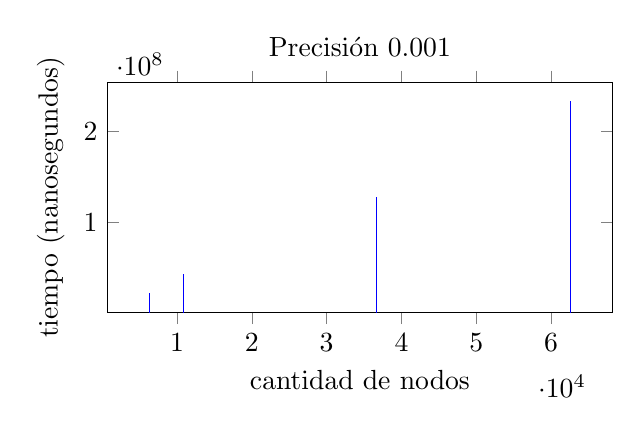
\begin{tikzpicture}
\begin{axis}[
    title=Precisión 0.001,
    xlabel=cantidad de nodos,
    ylabel=tiempo (nanosegundos),
    height=4.5cm, 
    width=8cm, 
    ybar, 
    bar width=5]
\addplot 
    coordinates {(6301,22337932.00) (10876,43180579.00) (36682,127379816.00) (62586,232454818.00)};

\end{axis}
\end{tikzpicture}
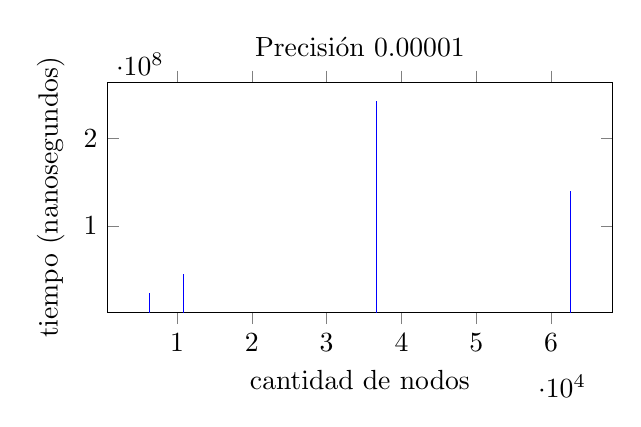
\begin{tikzpicture}
\begin{axis}[
    title=Precisión 0.00001,
    xlabel=cantidad de nodos,
    ylabel=tiempo (nanosegundos),
    height=4.5cm, 
    width=8cm, 
    ybar, 
    bar width=5]
\addplot 
    coordinates {(6301,22896544.00) (10876,43770720.00) (36682,242562037.00) (62586,140004295.00)};

\end{axis}
\end{tikzpicture}

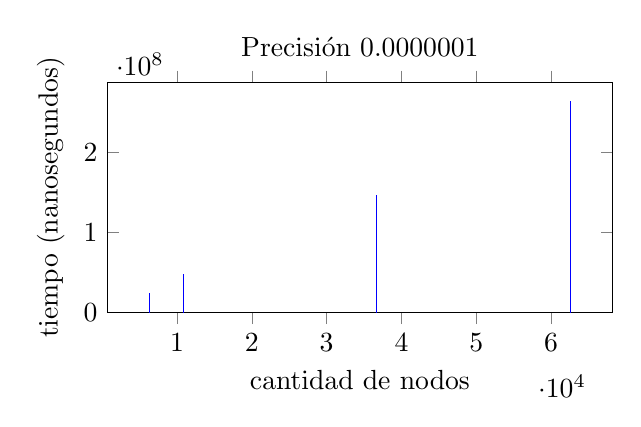
\begin{tikzpicture}
\begin{axis}[
    title=Precisión 0.0000001,
    xlabel=cantidad de nodos,
    ylabel=tiempo (nanosegundos),
    height=4.5cm, 
    width=8cm, 
    ybar, 
    bar width=5]
\addplot 
    coordinates {(6301,23884365.00) (10876,47676087.00) (36682,145804117.00) (62586,263878991.00)};

\end{axis}
\end{tikzpicture}
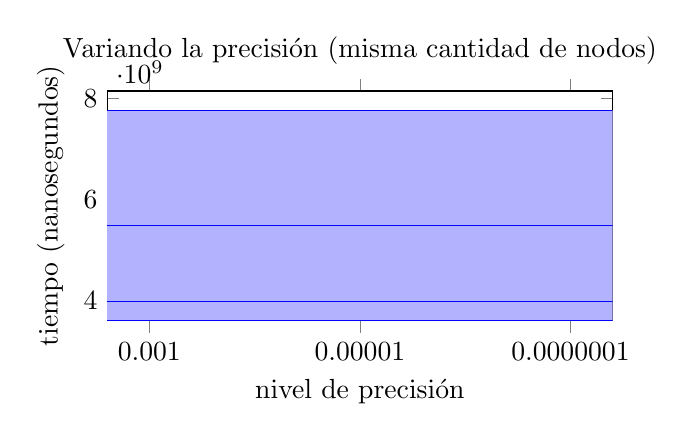
\begin{tikzpicture}
\begin{axis}[
    title=Variando la precisión (misma cantidad de nodos),
    xlabel=nivel de precisión,
    ylabel=tiempo (nanosegundos),
    xtick={1,2,3},
    xticklabels={0.001,0.00001,0.0000001},
    height=4.5cm, 
    width=8cm, 
    ybar, 
    bar width=10]
\addplot 
    coordinates {(1,3972349908.00) (2,5478391283.00) (3,7771818462.00)};

\end{axis}
\end{tikzpicture}


\subsubsection{Calidad de los resultados}

Para evaluar la calidad de las soluciones provistas por Page Rank las comparamos contra el algoritmo InDeg, que ordena las páginas según la cantidad de links que van hacia ellas.\\
Por el lado de Page Rank, no utilizamos la versión Esparsa del algoritmo, ya que el tamaño de la entrada no lo requiere.\\
Las instancias que usamos para hacer estas comparaciones fueron:
\begin{itemize}
    \item Instancia 1: 13 nodos y 18 ejes.
    \item Instancia 2: 13 nodos y 31 ejes.
    \item Instancia 3: 5 nodos y 20 ejes (grafo completo).
\end{itemize}
De forma de poder analizar los resultados facilmente, nos limitamos a instancias chicas.\\

Para la instancia 1, el valor $c$ del algoritmo Page Rank fue configurado en 0.3, 0.6 y luego en 0.9 con el fin de introducir la posibilidad de que el navegante salte a otra página de forma aleatoria y ver cuánto afecta al resultado final. Esto no es asi para la instancia 3 ya que al ser un grafo donde la probabilidad de ir a las demás páginas es igual para todas, el concepto de navegante aleatorio es irrelevante porque es igual de probable que vaya a cualquier página desde el principio.

Los resultados fueron:\newpage

\begin{center}
Instancia 1
\end{center}
\begin{figure}[H]
    \centering
    \begin{subfigure}[t]{0.5\textwidth}
      \begin{center}
        Page Rank(c = 0.3)\\
            \pgfplotstabletypeset[
                columns={rank,nodo,valor},
                columns/rank/.style={column name=Ranking},
                columns/nodo/.style={column name=Página},
                columns/valor/.style={column name=Importancia}
            ]{datos/pr-2-1-1.out}
      \end{center}
    \end{subfigure}%
    ~ 
    \begin{subfigure}[t]{0.5\textwidth}
      \begin{center}
        Page Rank(c = 0.6)\\
            \pgfplotstabletypeset[
                columns={rank,nodo,valor},
                columns/rank/.style={column name=Ranking},
                columns/nodo/.style={column name=Página},
                columns/valor/.style={column name=Importancia}
            ]{datos/pr-2-1-2.out}
      \end{center}
    \end{subfigure}
\end{figure}

\begin{figure}[H]
    \centering
    \begin{subfigure}[t]{0.5\textwidth}
      \begin{center}
        Page Rank(c = 0.9)\\
            \pgfplotstabletypeset[
                columns={rank,nodo,valor},
                columns/rank/.style={column name=Ranking},
                columns/nodo/.style={column name=Página},
                columns/valor/.style={column name=Importancia}
            ]{datos/pr-2-1-3.out}
      \end{center}
    \end{subfigure}%
    ~ 
    \begin{subfigure}[t]{0.5\textwidth}
      \begin{center}
        InDeg\\
            \pgfplotstabletypeset[
                columns={rank,nodo,valor},
                columns/rank/.style={column name=Ranking},
                columns/nodo/.style={column name=Página},
                columns/valor/.style={column name=In Degree}
            ]{datos/pr-2-1-4.out}
      \end{center}
    \end{subfigure}
\end{figure}

Por un lado, Page Rank obtiene un ranking con valores lógicos en el sentido de que el nodo con mas ejes hacia él es el de mayor importancia y los nodos con cantidad de links parecidos reciben un ranking similar.\\
Como podemos ver, los resultados de Page Rank no varian mucho, sus valores son afectados pero los rankings varian muy levemente. Esto es debido a que la cantidad de ejes no es de un tamaño tan grande como para que la variación de $c$ afecte el ranking.\\
A su vez, InDeg da los resultados que esperabamos, ordenando según la cantidad de links entrantes.\\
En comparación, los algoritmos dan resultados parecidos de a secciones pero sí tiene diferencias en los primeros puestos. Esto se debe a que Page Rank detecta que por las probabilildades del recorrido que un navegante puede hacer, no necesariamente las páginas con mas links entrantes van a ser las más visitadas a futuro.\\

Aun asi, veamos otro ejemplo donde la cantidad de ejes sea un poco mayor:

\begin{center}
Instancia 2
\end{center}

\begin{figure}[H]
    \centering
    \begin{subfigure}[t]{0.5\textwidth}
      \begin{center}
        Page Rank(c = 0.3)\\
            \pgfplotstabletypeset[
                columns={rank,nodo,valor},
                columns/rank/.style={column name=Ranking},
                columns/nodo/.style={column name=Página},
                columns/valor/.style={column name=Importancia}
            ]{datos/pr-2-2-1.out}
      \end{center}
    \end{subfigure}%
    ~ 
    \begin{subfigure}[t]{0.5\textwidth}
      \begin{center}
        Page Rank(c = 0.6)\\
            \pgfplotstabletypeset[
                columns={rank,nodo,valor},
                columns/rank/.style={column name=Ranking},
                columns/nodo/.style={column name=Página},
                columns/valor/.style={column name=Importancia}
            ]{datos/pr-2-2-2.out}
      \end{center}
    \end{subfigure}
\end{figure}

\begin{figure}[H]
    \centering
    \begin{subfigure}[t]{0.5\textwidth}
      \begin{center}
        Page Rank(c = 0.9)\\
            \pgfplotstabletypeset[
                columns={rank,nodo,valor},
                columns/rank/.style={column name=Ranking},
                columns/nodo/.style={column name=Página},
                columns/valor/.style={column name=Importancia}
            ]{datos/pr-2-2-3.out}
      \end{center}
    \end{subfigure}%
    ~ 
    \begin{subfigure}[t]{0.5\textwidth}
      \begin{center}
        InDeg\\
            \pgfplotstabletypeset[
                columns={rank,nodo,valor},
                columns/rank/.style={column name=Ranking},
                columns/nodo/.style={column name=Página},
                columns/valor/.style={column name=In Degree}
            ]{datos/pr-2-2-4.out}
      \end{center}
    \end{subfigure}
\end{figure}

En este caso ya podemos ver que el ranking varía más. Esto se debe a que ahora la cantidad de ejes es mayor con respecto a la cantidad de vértices. Por lo tanto, cuando vamos variando $c$, el algoritmo devuelve diferentes respuestas porque ahora la distribución de los links cobra más relevancia a comparación del factor "navegante aleatorio".\\
A diferencia del caso anterior, los resultados ya no son tan parecidos a los del algoritmo InDeg. De hecho, en solo un caso coincide PageRank con InDeg en el primer puesto del ranking. Lo que sugiere que la distribución de los ejes y su cantidad afectan la impredecibilidad del resultado.\\
Además, los ejes están distribuidos de tal manera que no haya grupos grandes aislados o grafos completos donde un grupo de vértices tenga una distribución de probabilidad muy pareja y nada de relación con otras componentes conexas.\\
Para ilustrar este caso veamos el siguiente ejemplo de un grafo completo:

\begin{center}
Instancia 3
\end{center}

\begin{figure}[H]
    \centering
    \begin{subfigure}[t]{0.5\textwidth}
      \begin{center}
        Page Rank\\
            \pgfplotstabletypeset[
                columns={rank,nodo,valor},
                columns/rank/.style={column name=Ranking},
                columns/nodo/.style={column name=Página},
                columns/valor/.style={column name=Importancia}
            ]{datos/pr-2-3-1.out}
      \end{center}
    \end{subfigure}%
    ~ 
    \begin{subfigure}[t]{0.5\textwidth}
      \begin{center}
        InDeg\\
            \pgfplotstabletypeset[
                columns={rank,nodo,valor},
                columns/rank/.style={column name=Ranking},
                columns/nodo/.style={column name=Página},
                columns/valor/.style={column name=In Degree}
            ]{datos/pr-2-3-2.out}
      \end{center}
    \end{subfigure}
\end{figure}

Los resultados indican lo lógico, como es un grafo donde la probabilidad de ir a cualquier lado es igual, tanto Page Rank como InDeg resuelven el problema asignandole igual importancia a cada página.\\
Por lo tanto concluimos que tanto la cantidad de ejes como la distribución son los factores que más contribuyen a los resultados de Page Rank.

\subsection{GeM}

\subsubsection{Variando el parámetro $c$}\label{exp_gem_2}
Este experimento consite en variar el parámetro $c$ y analizar como impacta esta
variación en los resultados obtenidos al generar el ranking con GeM.

Recordemos que $c$ es el coeficiente de amortiguación, que regula que tanto afecta
el \textit{navegante aleatorio} al resultado final.

Como es intuitivo de pensar, nuestra hipotesis en este experimento es que al tender
$c$ a cero aumenta la influencia del \textit{navegante aleatorio} en el puntaje de
cada página y, por lo tanto, más se parecen los puntajes de todas la páginas.
Es decir, menos dejan de importar los links salientes de las distintas páginas
del grafo original.

Por otro lado, cuando $c$ tiende a uno se debilita la influencia del \textit{navegante
aleatorio}, causando que el puntaje dependa solo de la matriz $H + au^{t}$, descrita
en la sección \ref{sec:gem_model}.

Se muestran a continuación dichos resultados para diferentes valores de $c$:

\begin{table}[H]
    \begin{center}
        \begin{tabular}{| c | l | c |}
            \hline
            Posicion & Equipo & Puntaje \\ \hline
            1 & Vélez Sarsfield & 0.033333 \\
            2 & Unión & 0.033333 \\
            3 & Gimnasia y Esgrima (LP) & 0.033333 \\
            4 & Estudiantes (LP) & 0.033333 \\
            5 & Defensa y Justicia & 0.033333 \\
            6 & Crucero del Norte & 0.033333 \\
            7 & Colón & 0.033333 \\
            \vdots & \quad\vdots & \vdots \\
            24 & Lanús & 0.033333 \\
            25 & San Lorenzo & 0.033333 \\
            26 & Rosario Central & 0.033333 \\
            27 & River Plate & 0.033333 \\
            28 & Racing Club & 0.033333 \\
            29 & Quilmes & 0.033333 \\
            30 & Olimpo & 0.033333 \\
            \hline
        \end{tabular}
        \begin{tabular}{| c | l | c |}
            \hline
            Posicion & Equipo & Puntaje \\ \hline
            1 & Boca Juniors & 0.051301 \\
            2 & San Lorenzo & 0.044563 \\
            3 & River Plate & 0.044200 \\
            4 & Racing Club & 0.040067 \\
            5 & Aldosivi & 0.039451 \\
            6 & Rosario Central & 0.039114 \\
            7 & Quilmes & 0.036699 \\
            \vdots & \quad\vdots & \vdots \\
            24 & Godoy Cruz & 0.028356 \\
            25 & Argentinos Juniors & 0.028208 \\
            26 & Temperley & 0.027904 \\
            27 & Crucero del Norte & 0.027353 \\
            28 & Nueva Chicago & 0.026346 \\
            29 & Atlético de Rafaela & 0.025776 \\
            30 & Colón & 0.025577 \\
            \hline
        \end{tabular}
        \captionsetup{justification=centering}
        \caption{A izquierda: puntajes obtenidos con $c=0$, a derecha: puntajes obtenidos con $c=0.3$}
        \label{exp_resultados_variar_c_1}
    \end{center}
\end{table}

\begin{table}[H]
    \begin{center}
        \begin{tabular}{| c | l | c |}
            \hline
            Posicion & Equipo & Puntaje \\ \hline
            1 & Boca Juniors & 0.086019 \\
            2 & Aldosivi & 0.065353 \\
            3 & River Plate & 0.063500 \\
            4 & San Lorenzo & 0.062035 \\
            5 & Rosario Central & 0.048473 \\
            6 & Racing Club & 0.047878 \\
            7 & San Martín (SJ) & 0.043956 \\
            \vdots & \quad\vdots & \vdots \\
            24 & Godoy Cruz & 0.017516 \\
            25 & Temperley & 0.016045 \\
            26 & Crucero del Norte & 0.016039 \\
            27 & Argentinos Juniors & 0.015398 \\
            28 & Nueva Chicago & 0.014232 \\
            29 & Atlético de Rafaela & 0.011388 \\
            30 & Colón & 0.010276 \\
            \hline
        \end{tabular}
        \begin{tabular}{| c | l | c |}
            \hline
            Posicion & Equipo & Puntaje \\ \hline
            1 & Boca Juniors & 0.095290 \\
            2 & Aldosivi & 0.075151 \\
            3 & River Plate & 0.068142 \\
            4 & San Lorenzo & 0.065265 \\
            5 & Rosario Central & 0.050875 \\
            6 & Racing Club & 0.048824 \\
            7 & San Martín (SJ) & 0.047118 \\
            \vdots & \quad\vdots & \vdots \\
            24 & Godoy Cruz & 0.014148 \\
            25 & Crucero del Norte & 0.013132 \\
            26 & Temperley & 0.012487 \\
            27 & Argentinos Juniors & 0.011286 \\
            28 & Nueva Chicago & 0.011239 \\
            29 & Atlético de Rafaela & 0.007559 \\
            30 & Colón & 0.006003 \\
            \hline
        \end{tabular}
        \captionsetup{justification=centering}
        \caption{A izquierda: puntajes obtenidos con $c=0.85$, a derecha: puntajes obtenidos con $c=1$}
        \label{exp_resultados_variar_c_2}
    \end{center}
\end{table}

Analizando los resultados tenemos que:

\begin{itemize}
    \item Para $c=0$, la tabla de puntajes se condice con la hipótesis planteada.
        Los puntajes de los equipos no solo son parecidos, sino que son iguales.
        Y dicho puntaje es $0.0\hat{3} = 1/30 = 1/n$, dónde $n$ es la cantidad de
        equipos totales.
    \item A medida que el $c$ aumenta (desde $0.3$ a $1$) las posiciones van convergiendo.
        Ya con $c=0.3$, 6 de los 7 primeros equipos aparecen en los primeros 7 puestos con $c=1$,
        y los últimos 7 equipos con $c=0.3$ aparecen en los últimos 7 puestos con $c=1$.
    \item A su vez, la diferencia entre los resultados con $c=85$ y $c=1$ es muy chica:
        de los 14 equipos mostrados en el Cuadro \ref{exp_resultados_variar_c_2} solo dos
        de ellos cambian de posición (Crucero del Norte y Temperley).
\end{itemize}

En base a lo analizado, podemos concluir que los resultados del experimento corroboran
las hipotesis planteadas.

\subsubsection{Evolución del ranking}

\begin{center}
    \begin{tikzpicture}
    \begin{axis}[
        title={Evolución con GeM},
		xlabel=Fecha,
		ylabel=Puntaje,
		xmin=1,
		xmax=26,
		ymin=0,
		ymax=0.13,
        width=0.8\textwidth,
        height=0.5\textwidth,
		xtick={1,...,26},
		yticklabel style={/pgf/number format/fixed},
		legend style={at={(1.015,1)},anchor=north west},
		no markers,
		thick,
		cycle list name=exotic
    ]
    \addplot table[x index=0,y index=1]{../src/exp/gem-evolution-ranking.out};
    \addplot table[x index=0,y index=7]{../src/exp/gem-evolution-ranking.out};
    %\addplot table[x index=0,y index=17]{../src/exp/gem-evolution-ranking.out};
    \addplot table[x index=0,y index=20]{../src/exp/gem-evolution-ranking.out};
    \addplot table[x index=0,y index=21]{../src/exp/gem-evolution-ranking.out};
    \addplot table[x index=0,y index=22]{../src/exp/gem-evolution-ranking.out};
    \addplot table[x index=0,y index=23]{../src/exp/gem-evolution-ranking.out};
    \addplot table[x index=0,y index=24]{../src/exp/gem-evolution-ranking.out};
    \addplot table[x index=0,y index=25]{../src/exp/gem-evolution-ranking.out};
    %\addplot table[x index=0,y index=30]{../src/exp/gem-evolution-ranking.out};
	\legend{Aldosivi, Boca Juniors, Quilmes,
	Racing Club, River Plate, Rosario Central, San Lorenzo, San Martín (SJ)}
    \end{axis}
    \end{tikzpicture}
\end{center}

\begin{center}
    \begin{tikzpicture}
    \begin{axis}[
        title={Evolución con Puntaje AFA},
		xlabel=Fecha,
		ylabel=Puntaje,
		xmin=1,
		xmax=26,
		ymin=0,
		ymax=60,
        width=0.8\textwidth,
        height=0.5\textwidth,
		xtick={1,...,26},
		yticklabel style={/pgf/number format/fixed},
		legend style={at={(1.015,1)},anchor=north west},
		no markers,
		thick,
		cycle list name=exotic
    ]
	\addplot table[x index=0,y index=1]{../src/exp/afa-evolution-ranking.out};
    \addplot table[x index=0,y index=7]{../src/exp/afa-evolution-ranking.out};
    %\addplot table[x index=0,y index=17]{../src/exp/afa-evolution-ranking.out};
    \addplot table[x index=0,y index=20]{../src/exp/afa-evolution-ranking.out};
    \addplot table[x index=0,y index=21]{../src/exp/afa-evolution-ranking.out};
    \addplot table[x index=0,y index=22]{../src/exp/afa-evolution-ranking.out};
    \addplot table[x index=0,y index=23]{../src/exp/afa-evolution-ranking.out};
    \addplot table[x index=0,y index=24]{../src/exp/afa-evolution-ranking.out};
    \addplot table[x index=0,y index=25]{../src/exp/afa-evolution-ranking.out};
    %\addplot table[x index=0,y index=30]{../src/exp/afa-evolution-ranking.out};
	\legend{Aldosivi, Boca Juniors, Quilmes,
	Racing Club, River Plate, Rosario Central, San Lorenzo, San Martín (SJ)}
    \end{axis}
    \end{tikzpicture}
\end{center}

